% Provenance (never printed): old premiere S material on subduction (Wadati-Benioff
% planes, density of the old lithosphere, slab pull, transformation of the slab at
% depth: blueschist and eclogite; anatomy of an active margin). Sections from
% figdata/grade-11/slab_sections.py (USGS ComCat M >= 6 1976-2025, PB2002 steps,
% Seton 2020 ages); plate speeds from plate_velocities.py (NNR-MORVEL56 RMS).
% Metamorphism is defined in g12.03, the volcanic arc in g12.04: named only here.
\chapter{Subduction Zones}\label{ch:g11:subduction-zones}

Beneath the islands of Tonga, in the south-western Pacific, the Earth shakes
far deeper than anywhere else. Of the seven thousand earthquakes of magnitude
6 or more recorded worldwide between 1976 and 2025, the deepest happened
\qty{688}{km} down, and the section across Tonga in this chapter holds events down
to about \qty{671}{km}. At such depths the rock is hot and under enormous
pressure; it should flow slowly, like the \omterm{def:g11:lithosphere-asthenosphere:lithosphere}{asthenosphere}, not break. Yet it
breaks. This chapter explains what is there to break: a \omterm{def:g11:subduction-zones:slab}{slab} of cold ocean
floor, sinking back into the mantle.
% ledger: data:usgs-comcat (catalogue_maxdepth 688; tonga_maxdepth 670.8, slab_sections.py)

\begin{recall}
At a convergent boundary two plates move toward each other; deep trenches
line some of them (Book 1, grades 7 and 8). The magnitude of an earthquake
measures its size, and an earthquake under the sea can raise a tsunami
(Book 1, grade 7). The velocity of a plate relative to another is the
difference of their velocities (\cref{ch:g11:plate-motions}). Ocean floor
sinks as it ages, and after some 60 million years its \omterm{def:g11:lithosphere-asthenosphere:lithosphere}{lithosphere}, about
\qty{100}{km} thick, is denser than the \omterm{def:g11:lithosphere-asthenosphere:lithosphere}{asthenosphere} beneath it
(\cref{ch:g11:ocean-ridges}). Seismic waves show a sharp change in the mantle
at about \qty{670}{km} (\cref{ch:g11:seismic-structure}). A metamorphic rock
is a rock transformed in the solid state (Book 1, grade 6).
\end{recall}
% ledger: data:prem (670 km), ps77:depth-age

\section{Trenches and dipping earthquake zones}

Most earthquakes are shallow: in the catalogue of magnitude 6 or more since
1976, only about one in five is deeper than \qty{70}{km}, and one in fifteen
deeper than \qty{300}{km}. The map below shows where the deep ones are.
% values (slab_sections.py): frac_deeper_70 0.21, frac_deeper_300 0.069; data:usgs-comcat

\begin{omfigure}
\begin{tikzpicture}
\begin{axis}[ommap, width=\linewidth, xtick={-180,-90,...,180}, ytick={-60,0,60},
  legend style={font=\scriptsize, at={(0.5,-0.13)}, anchor=north, legend columns=3,
    /tikz/every even column/.append style={column sep=6pt}}]
\addplot[fill=omLithAlluv, draw=black!45, line width=0.2pt, forget plot] table {figdata/out/shared-geo-land.dat};
\addplot[black!70, line width=0.5pt, forget plot] table {figdata/out/shared-geo-school-subduction.dat};
\addplot[fill=black!70, draw=none, forget plot] table {figdata/out/shared-geo-school-teeth.dat};
% computed in figdata/grade-11/slab_sections.py; ledger: data:usgs-comcat, data:pb2002
\addplot[only marks, mark=*, mark size=0.55pt, black!45] table[x=lon, y=lat] {figdata/out/grade-11-slab_sections-world-shallow.dat};
\addplot[only marks, mark=*, mark size=0.8pt, omProp] table[x=lon, y=lat] {figdata/out/grade-11-slab_sections-world-mid.dat};
\addplot[only marks, mark=*, mark size=1.1pt, omThm] table[x=lon, y=lat] {figdata/out/grade-11-slab_sections-world-deep.dat};
\legend{{shallower than \qty{70}{km}}, {70 to \qty{300}{km}}, {deeper than \qty{300}{km}}}
\end{axis}
\end{tikzpicture}

{\small Earthquakes of magnitude 6.5 or more, 1976--2025 (2192 events),
coloured by depth, with the trenches (black line, triangles on the plate that
overrides). Intermediate and deep earthquakes lie only along some trenches,
always on the side of the overriding plate. Data: USGS earthquake catalogue;
plate boundaries of Bird (2003); land from Natural Earth.}
\end{omfigure}
% values: world_n_m65 2192, world_deep_n 197 (slab_sections.py)

The deep earthquakes are not scattered: they follow the trenches of the
western Pacific, from Kamchatka to Japan, the Marianas, Indonesia and Tonga,
and the trench along the west coast of South America; and they always lie on
one side of the trench, under the plate that does not sink.

\begin{definition}[Subduction; subduction zone]\label{def:g11:subduction-zones:subduction}
\emph{Subduction}\index{subduction} is the sinking of a plate of \omterm{def:g11:ocean-ridges:oceanic-lithosphere}{oceanic
lithosphere} beneath another plate, back into the mantle. A \emph{subduction
zone}\index{subduction zone} is a convergent plate boundary where subduction
takes place; it is marked at the surface by a trench.
\end{definition}

\begin{definition}[Wadati--Benioff zone]\label{def:g11:subduction-zones:benioff}
A \emph{Wadati--Benioff zone}\index{Wadati--Benioff zone} is the inclined
band of earthquakes that starts at a trench and goes deeper and deeper beneath
the overriding plate, down to as much as about \qty{700}{km}.
\end{definition}
% ledger: frohlich87:wadati

\begin{history}[Wadati and Benioff]
In the 1920s leading seismologists argued that earthquakes could happen
only in the first few tens of kilometres: the deeper Earth, they reasoned,
had no strength to store the strain. The Japanese seismologist Kiyoo Wadati, who worked with the
dense network of stations of the Japan Meteorological Agency, gave from 1928
the first convincing evidence that some earthquakes are hundreds of
kilometres deep: one of the events he studied, in January 1927, was
\qty{420}{km} down. In 1935 he published the first map of the depths of
these earthquakes, drawn as contour lines, and noticed that the deepening
zone ran parallel to the line of active volcanoes. In 1949 and 1954 the
American seismologist Hugo Benioff showed that beneath the Andes and the
Tonga--Kermadec islands the earthquakes lie along zones reaching depths of
about \qty{700}{km}. The zones were first called Benioff zones, in 1967; the
name \omterm{def:g11:subduction-zones:benioff}{Wadati--Benioff zone}, which gives both their due, follows a suggestion
of the Japanese geophysicist Seiya Uyeda in 1971.
\end{history}
% ledger: frohlich87:wadati

\begin{method}[Reading an earthquake section]\label{met:g11:subduction-zones:section}
\begin{enumerate}
  \item Choose a line perpendicular to the trench, from the trench toward the
        overriding plate, and keep the earthquakes within a band on either
        side of it.
  \item Plot each earthquake at its distance along the line (horizontally)
        and at its depth (vertically, downward).
  \item Look for the inclined band; draw the straight line that follows it
        best.
  \item Read the dip of the band from two points of the line (proposition
        below).
\end{enumerate}
\end{method}

\begin{omfigure}
\begin{tikzpicture}
\begin{axis}[omrecord, omdepth, name=tonga, width=0.5\linewidth, height=6.4cm,
  xmin=-150, xmax=900, ymin=0, ymax=720, xlabel={distance from the trench (\unit{km})},
  ylabel={depth (\unit{km})}, title={\small Tonga}, clip=false]
% computed in figdata/grade-11/slab_sections.py; ledger: data:usgs-comcat, data:pb2002
\addplot[only marks, mark=*, mark size=1.2pt, black!65] table[x=x, y=depth] {figdata/out/grade-11-slab_sections-tonga.dat};
\addplot[omProp, line width=1pt, domain=135.7:761.6, samples=2] {-23.568 + 0.91068*x};
\addplot[only marks, mark=triangle*, mark size=3pt, omDef] coordinates {(0,0)};
\node[font=\scriptsize, anchor=south west, text=omDef] at (axis cs:10,8) {trench};
\node[font=\scriptsize, anchor=west, text=omProp, align=left] at (axis cs:300,560) {dip\\\ang{42}};
\end{axis}
\begin{axis}[omrecord, omdepth, at={(tonga.east)}, anchor=west, xshift=0.3cm, width=0.5\linewidth, height=6.4cm,
  xmin=-150, xmax=900, ymin=0, ymax=720, xlabel={distance from the trench (\unit{km})},
  yticklabels={}, title={\small Andes, near \ang{21} South}, clip=false]
\addplot[only marks, mark=*, mark size=1.2pt, black!65] table[x=x, y=depth] {figdata/out/grade-11-slab_sections-andes.dat};
\addplot[omProp, line width=1pt, domain=253.0:900, samples=2] {-88.745 + 0.74613*x};
\addplot[only marks, mark=triangle*, mark size=3pt, omDef] coordinates {(0,0)};
\node[font=\scriptsize, anchor=south west, text=omDef] at (axis cs:10,8) {trench};
\node[font=\scriptsize, anchor=west, text=omProp, align=left] at (axis cs:300,560) {dip\\\ang{37}};
\end{axis}
\end{tikzpicture}

{\small Earthquake sections perpendicular to two trenches: earthquakes of
magnitude 6 or more, 1976--2025, within \qty{150}{km} of the section line,
plotted at their distance from the trench (toward the overriding plate) and
their depth. Orange: the straight line that best follows the earthquakes
between 100 and \qty{600}{km} deep. Beneath Tonga the band reaches below
\qty{670}{km}. Data: USGS earthquake catalogue; trench positions from Bird (2003).}
\end{omfigure}
% values (slab_sections.py): tonga_dip 42.3, fit -23.568 + 0.91068 x (77 events);
% andes_dip 36.7, fit -88.745 + 0.74613 x; trench points tonga (-173.31, -20.395),
% andes (-71.286, -21.01)

\begin{proposition}[The dip of a slab from an earthquake section]\label{prop:g11:subduction-zones:dip}
If two points of the line that follows a \omterm{def:g11:subduction-zones:benioff}{Wadati--Benioff zone} lie at
horizontal distances $x_1 < x_2$ from the trench and depths $z_1$ and $z_2$,
its dip $\delta$, the angle it makes with the horizontal, satisfies
\[
  \tan \delta = \frac{z_2 - z_1}{x_2 - x_1}.
\]
\end{proposition}

\begin{proof}
The two points and the point at depth $z_1$ vertically above the second one
form a right triangle. Its horizontal side is $x_2 - x_1$, its vertical side
$z_2 - z_1$, and the angle at the first point is the dip. The tangent of an
angle of a right triangle is the opposite side over the adjacent side.
\end{proof}

\begin{example}[The dip beneath Tonga]\label{ex:g11:subduction-zones:dip}
The line of the Tonga section passes \qty{250}{km} down at \qty{300}{km} from
the trench and \qty{614}{km} down at \qty{700}{km}. So
$\tan\delta = (614 - 250)/(700 - 300) = 364/400 = 0.91$, and
$\delta \approx \ang{42}$. Beneath the Andes, at \ang{21}~South, the same
method gives about \ang{37}.
\end{example}
% values: tonga line at 300 km 249.6, at 700 km 613.9 (slab_sections.py)

The \omterm{def:g11:subduction-zones:benioff}{Wadati--Benioff zone} traces a plate that goes down. Shallow earthquakes
happen where the two plates slide against each other, near the trench; deeper
ones happen inside the sinking plate itself.

\section{Why old lithosphere sinks}

\begin{definition}[Slab]\label{def:g11:subduction-zones:slab}
A \emph{slab}\index{slab} is the part of a plate that has already sunk into
the mantle at a \omterm{def:g11:subduction-zones:subduction}{subduction zone}: a sheet of \omterm{def:g11:ocean-ridges:oceanic-lithosphere}{oceanic lithosphere}, about a
hundred kilometres thick, inclined beneath the overriding plate.
\end{definition}

What goes down is old ocean floor. From the age of the ocean floor, the floor
that reaches the Japan Trench, east of Japan, is about 133 million years old,
the floor that reaches the Tonga Trench about 99 million years old; even the
floor that reaches the Andes, among the youngest to sink, is about 49
million years old. Such old \omterm{def:g11:lithosphere-asthenosphere:lithosphere}{lithosphere} is cold and thick, and, apart from
its light crust, denser than the \omterm{def:g11:lithosphere-asthenosphere:lithosphere}{asthenosphere}: as soon as one edge of it
starts to go down, its own weight pulls it in.
% values (slab_sections.py): japan_age 133.1, tonga_age 98.8, andes_age 48.8 (median of the
% 1-degree cells 100-400 km seaward of the trench point); ledger data:b2-seafloor-age

\begin{definition}[Slab pull; ridge push]\label{def:g11:subduction-zones:slab-pull}
\emph{Slab pull}\index{slab pull} is the force that a sinking \omterm{def:g11:subduction-zones:slab}{slab}, denser
than the mantle around it, exerts on the rest of its plate, pulling it toward
the trench. \emph{Ridge push}\index{ridge push} is the force that pushes a
plate away from a ridge, where the young, hot \omterm{def:g11:lithosphere-asthenosphere:lithosphere}{lithosphere} stands high on its
raised ridge and slides down its slope.
\end{definition}

Which of the two matters more? In 1975 Donald Forsyth and Seiya Uyeda
worked out the strength of each force from the speeds and the shapes of
the plates: the forces on the sinking \omterm{def:g11:subduction-zones:slab}{slabs} control the speed of the oceanic plates,
and are about ten times stronger than any other force. Today's plate
velocities show it clearly.
% ledger: fu75:slab-pull

\begin{omfigure}
\begin{tikzpicture}
\begin{axis}[omrecord, ybar, bar width=9pt, width=0.86\linewidth, height=5.6cm,
  ymin=0, ymax=85, xmin=-0.7, xmax=12.7, bar shift=0pt, ylabel={mean speed (\unit{mm} a year)},
  xtick={0,...,12}, xticklabel style={rotate=50, anchor=east, font=\scriptsize},
  xticklabels={Cocos, Nazca, Pacific, Australia, Philippine Sea, Arabia, Somalia,
    Nubia, Eurasia, North America, Antarctica, Caribbean, South America},
  ymajorgrids, xmajorgrids=false]
% computed in figdata/grade-11/slab_sections.py from plate_velocities.POLES (nnr56:rms)
\addplot[fill=omProp, draw=omProp!70!black] table[x=idx, y expr=\thisrow{slab}*\thisrow{rms}] {figdata/out/grade-11-slab_sections-speeds.dat};
\addplot[fill=omDef!35, draw=omDef] table[x=idx, y expr=(1-\thisrow{slab})*\thisrow{rms}] {figdata/out/grade-11-slab_sections-speeds.dat};
\node[font=\scriptsize, text=omProp!80!black, anchor=south] at (axis cs:2,76) {a slab hangs from the plate};
\node[font=\scriptsize, text=omDef, anchor=south] at (axis cs:9,50) {no long slab};
\end{axis}
\end{tikzpicture}

{\small The mean speed of thirteen large plates (root mean square over
the plate, in a frame in which the \omterm{def:g11:lithosphere-asthenosphere:lithosphere}{lithosphere} as a whole does not turn).
Orange: plates from which a sinking \omterm{def:g11:subduction-zones:slab}{slab} hangs along a long stretch of edge;
blue: plates without one. India is left out: its northern edge is a
collision. Data: NNR-MORVEL56 (Argus, Gordon and DeMets,
2011).}
\end{omfigure}
% ledger: nnr56:rms; the bars of a class are drawn at 0 for the other (two series on one axis)

\begin{proposition}[Plates attached to slabs are fast]\label{prop:g11:subduction-zones:fast}
The five large plates from which a long \omterm{def:g11:subduction-zones:slab}{slab} hangs (Cocos, Nazca, Pacific,
Australia, Philippine Sea) move on average at about \qty{65}{mm} a year; the
eight without one at about \qty{24}{mm} a year, nearly three times slower.
Each plate of the first group is faster than every plate of the second.
\end{proposition}
% values: rms_slab_mean 65.2, rms_noslab_mean 23.9 (plate_velocities.py); India left out
% (its northern edge is a collision)

\begin{proof}
From the published mean speeds, the \omterm{def:g11:subduction-zones:slab}{slab} plates give
$(74.6 + 70.0 + 65.5 + 63.1 + 52.6)/5 \approx 65.2$ and the others
$(47.6 + 31.0 + 29.2 + 22.8 + 19.8 + 15.2 + 14.9 + 10.6)/8 \approx 23.9$
(millimetres a year); the slowest \omterm{def:g11:subduction-zones:slab}{slab} plate, the Philippine Sea plate at
52.6, is faster than the fastest of the others, Arabia at 47.6.
\end{proof}
% ledger: nnr56:rms

\section{The slab transformed at depth}

As the \omterm{def:g11:subduction-zones:slab}{slab} goes down, its crust of basalt and \omterm{def:g11:ocean-ridges:gabbro}{gabbro} is buried deeper and
deeper while staying cold, since the \omterm{def:g11:subduction-zones:slab}{slab} sinks faster than heat can reach its
interior. The rocks of the crust change their minerals without melting: they
are metamorphosed (\cref{ch:g12:metamorphic-rocks}). Two rocks mark the path.

\begin{definition}[Blueschist; eclogite]\label{def:g11:subduction-zones:eclogite}
\emph{Blueschist}\index{blueschist} is a metamorphic rock made from basalt
of the \omterm{def:g11:ocean-ridges:oceanic-lithosphere}{oceanic crust} buried to high pressure while it stays relatively cold;
it is coloured blue by the mineral glaucophane. \emph{Eclogite}\index{eclogite}
is the dense metamorphic rock that basalt and \omterm{def:g11:ocean-ridges:gabbro}{gabbro} become at mantle depths
along \omterm{def:g11:subduction-zones:subduction}{subduction zones}: it has the same chemical composition, but is made of
red garnet and green pyroxene.
\end{definition}
% ledger: photo:g11-blueschist, photo:g11-eclogite

\begin{omfigure}
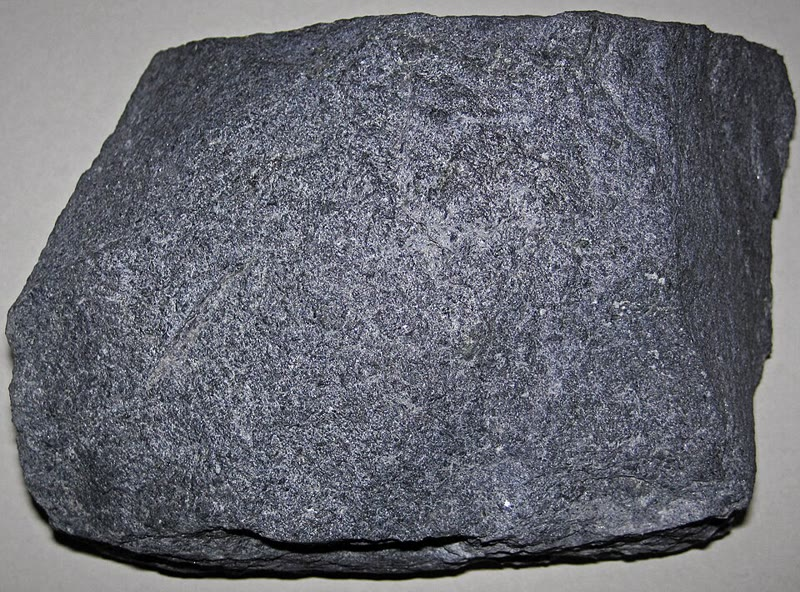
\includegraphics[height=4.4cm]{images/book2/g11-stjohn-blueschist.jpg}\hspace{0.03\linewidth}%
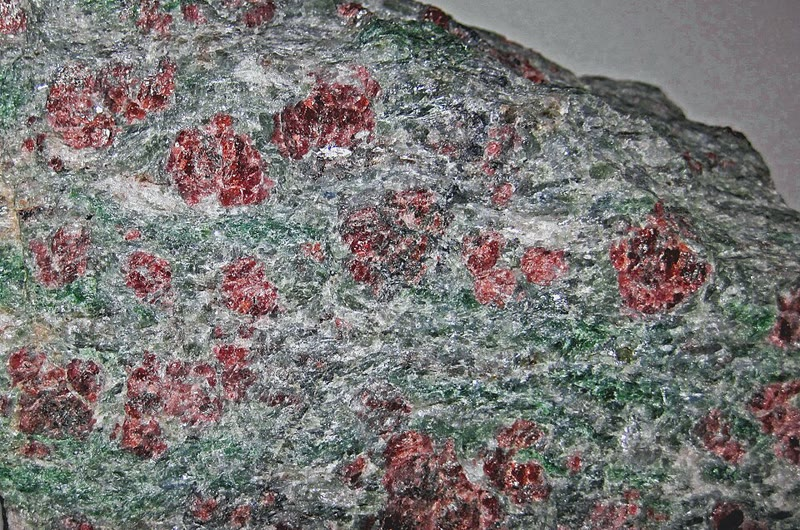
\includegraphics[height=4.4cm]{images/book2/g11-stjohn-eclogite.jpg}

{\small Left: \omterm{def:g11:subduction-zones:eclogite}{blueschist} from Santa Catalina Island, California, once \omterm{def:g11:ocean-ridges:oceanic-lithosphere}{oceanic
crust} buried in a \omterm{def:g11:subduction-zones:subduction}{subduction zone}. Right: \omterm{def:g11:subduction-zones:eclogite}{eclogite} from Norway, with red
garnets in green pyroxene. Photographs James St.~John (CC~BY~2.0).}
\end{omfigure}
% ledger: photo:g11-blueschist, photo:g11-eclogite

\omterm{def:g11:subduction-zones:eclogite}{Eclogite} is denser than basalt; it is even denser than the \omterm{def:g11:ocean-ridges:peridotite}{peridotite} of the
mantle, by about \qty{6}{\percent}. Once its crust has turned into \omterm{def:g11:subduction-zones:eclogite}{eclogite},
the \omterm{def:g11:subduction-zones:slab}{slab} no longer carries a light layer on top: the whole \omterm{def:g11:subduction-zones:slab}{slab} is denser
than the mantle around it, and pulls harder. Rocks of this kind, brought back
to the surface by later movements, are among the few direct witnesses of
what happens tens of kilometres down in a \omterm{def:g11:subduction-zones:subduction}{subduction zone}.
% ledger: hacker03:eclogite, photo:g11-eclogite

\begin{omfigure}
\begin{tikzpicture}[font=\footnotesize, scale=0.85]
  % subduction zone, a drawing, not to scale: slab top flat to x = -1, then bends to a 42-degree dip
  % coordinates computed once by a small script (scratch, not kept): slab top flat to x=-1, arc R=3 to a 42-degree dip
  \fill[omProp!10] (-7,-1.4) rectangle (7,-6.0);
  \fill[omSea!45] (-7,0) -- (-1,0) -- (1.6,0.8) -- (-7,0.8) -- cycle;
  \fill[lith peridotite] (-7.000,0.000) -- (-6.644,0.000) -- (-6.289,0.000) -- (-5.933,0.000) -- (-5.578,0.000) -- (-5.222,0.000) -- (-4.867,0.000) -- (-4.511,0.000) -- (-4.156,0.000) -- (-3.800,0.000) -- (-3.445,0.000) -- (-3.089,0.000) -- (-2.734,0.000) -- (-2.378,0.000) -- (-2.023,0.000) -- (-1.667,0.000) -- (-1.312,0.000) -- (-0.956,-0.000) -- (-0.602,-0.027) -- (-0.253,-0.094) -- (0.085,-0.203) -- (0.408,-0.351) -- (0.712,-0.536) -- (0.991,-0.756) -- (1.255,-0.994) -- (1.519,-1.232) -- (1.784,-1.470) -- (2.048,-1.707) -- (2.312,-1.945) -- (2.576,-2.183) -- (2.840,-2.421) -- (3.105,-2.659) -- (3.369,-2.897) -- (3.633,-3.135) -- (3.897,-3.373) -- (4.161,-3.611) -- (4.426,-3.848) -- (4.690,-4.086) -- (4.954,-4.324) -- (5.218,-4.562) -- (5.483,-4.800) -- (4.546,-5.840) -- (4.282,-5.603) -- (4.017,-5.365) -- (3.753,-5.127) -- (3.489,-4.889) -- (3.225,-4.651) -- (2.961,-4.413) -- (2.696,-4.175) -- (2.432,-3.937) -- (2.168,-3.699) -- (1.904,-3.461) -- (1.639,-3.224) -- (1.375,-2.986) -- (1.111,-2.748) -- (0.847,-2.510) -- (0.583,-2.272) -- (0.318,-2.034) -- (0.062,-1.803) -- (-0.087,-1.686) -- (-0.249,-1.587) -- (-0.421,-1.508) -- (-0.602,-1.450) -- (-0.788,-1.414) -- (-0.977,-1.400) -- (-1.312,-1.400) -- (-1.667,-1.400) -- (-2.023,-1.400) -- (-2.378,-1.400) -- (-2.734,-1.400) -- (-3.089,-1.400) -- (-3.445,-1.400) -- (-3.800,-1.400) -- (-4.156,-1.400) -- (-4.511,-1.400) -- (-4.867,-1.400) -- (-5.222,-1.400) -- (-5.578,-1.400) -- (-5.933,-1.400) -- (-6.289,-1.400) -- (-6.644,-1.400) -- (-7.000,-1.400) -- cycle;
  \fill[lith basalt] (-7.000,0.000) -- (-6.644,0.000) -- (-6.289,0.000) -- (-5.933,0.000) -- (-5.578,0.000) -- (-5.222,0.000) -- (-4.867,0.000) -- (-4.511,0.000) -- (-4.156,0.000) -- (-3.800,0.000) -- (-3.445,0.000) -- (-3.089,0.000) -- (-2.734,0.000) -- (-2.378,0.000) -- (-2.023,0.000) -- (-1.667,0.000) -- (-1.312,0.000) -- (-0.956,-0.000) -- (-0.602,-0.027) -- (-0.253,-0.094) -- (0.085,-0.203) -- (0.408,-0.351) -- (0.712,-0.536) -- (0.991,-0.756) -- (1.255,-0.994) -- (1.519,-1.232) -- (1.784,-1.470) -- (2.048,-1.707) -- (2.312,-1.945) -- (2.576,-2.183) -- (2.840,-2.421) -- (3.105,-2.659) -- (3.369,-2.897) -- (3.633,-3.135) -- (3.897,-3.373) -- (4.161,-3.611) -- (4.426,-3.848) -- (4.690,-4.086) -- (4.954,-4.324) -- (5.218,-4.562) -- (5.483,-4.800) -- (5.282,-5.023) -- (5.018,-4.785) -- (4.753,-4.547) -- (4.489,-4.309) -- (4.225,-4.071) -- (3.961,-3.833) -- (3.697,-3.596) -- (3.432,-3.358) -- (3.168,-3.120) -- (2.904,-2.882) -- (2.640,-2.644) -- (2.376,-2.406) -- (2.111,-2.168) -- (1.847,-1.930) -- (1.583,-1.692) -- (1.319,-1.455) -- (1.054,-1.217) -- (0.792,-0.980) -- (0.541,-0.783) -- (0.268,-0.616) -- (-0.023,-0.483) -- (-0.328,-0.385) -- (-0.642,-0.324) -- (-0.960,-0.300) -- (-1.312,-0.300) -- (-1.667,-0.300) -- (-2.023,-0.300) -- (-2.378,-0.300) -- (-2.734,-0.300) -- (-3.089,-0.300) -- (-3.445,-0.300) -- (-3.800,-0.300) -- (-4.156,-0.300) -- (-4.511,-0.300) -- (-4.867,-0.300) -- (-5.222,-0.300) -- (-5.578,-0.300) -- (-5.933,-0.300) -- (-6.289,-0.300) -- (-6.644,-0.300) -- (-7.000,-0.300) -- cycle;
  \fill[blue!30] (2.484,-2.100) -- (2.604,-2.208) -- (2.725,-2.317) -- (2.845,-2.425) -- (2.965,-2.533) -- (3.085,-2.642) -- (3.206,-2.750) -- (3.326,-2.858) -- (3.446,-2.967) -- (3.567,-3.075) -- (3.687,-3.183) -- (3.807,-3.292) -- (3.928,-3.400) -- (3.727,-3.623) -- (3.607,-3.515) -- (3.486,-3.406) -- (3.366,-3.298) -- (3.246,-3.190) -- (3.125,-3.081) -- (3.005,-2.973) -- (2.885,-2.865) -- (2.764,-2.756) -- (2.644,-2.648) -- (2.524,-2.540) -- (2.403,-2.431) -- (2.283,-2.323) -- cycle;
  \fill[lith eclogite] (3.928,-3.400) -- (4.057,-3.517) -- (4.187,-3.633) -- (4.316,-3.750) -- (4.446,-3.867) -- (4.576,-3.983) -- (4.705,-4.100) -- (4.835,-4.217) -- (4.964,-4.333) -- (5.094,-4.450) -- (5.223,-4.567) -- (5.353,-4.683) -- (5.483,-4.800) -- (5.282,-5.023) -- (5.152,-4.906) -- (5.023,-4.790) -- (4.893,-4.673) -- (4.764,-4.556) -- (4.634,-4.440) -- (4.504,-4.323) -- (4.375,-4.206) -- (4.245,-4.090) -- (4.116,-3.973) -- (3.986,-3.856) -- (3.857,-3.740) -- (3.727,-3.623) -- cycle;
  \draw[black!60] (-7.000,0.000) -- (-6.644,0.000) -- (-6.289,0.000) -- (-5.933,0.000) -- (-5.578,0.000) -- (-5.222,0.000) -- (-4.867,0.000) -- (-4.511,0.000) -- (-4.156,0.000) -- (-3.800,0.000) -- (-3.445,0.000) -- (-3.089,0.000) -- (-2.734,0.000) -- (-2.378,0.000) -- (-2.023,0.000) -- (-1.667,0.000) -- (-1.312,0.000) -- (-0.956,-0.000) -- (-0.602,-0.027) -- (-0.253,-0.094) -- (0.085,-0.203) -- (0.408,-0.351) -- (0.712,-0.536) -- (0.991,-0.756) -- (1.255,-0.994) -- (1.519,-1.232) -- (1.784,-1.470) -- (2.048,-1.707) -- (2.312,-1.945) -- (2.576,-2.183) -- (2.840,-2.421) -- (3.105,-2.659) -- (3.369,-2.897) -- (3.633,-3.135) -- (3.897,-3.373) -- (4.161,-3.611) -- (4.426,-3.848) -- (4.690,-4.086) -- (4.954,-4.324) -- (5.218,-4.562) -- (5.483,-4.800);
  \draw[black!60] (-7.000,-1.400) -- (-6.644,-1.400) -- (-6.289,-1.400) -- (-5.933,-1.400) -- (-5.578,-1.400) -- (-5.222,-1.400) -- (-4.867,-1.400) -- (-4.511,-1.400) -- (-4.156,-1.400) -- (-3.800,-1.400) -- (-3.445,-1.400) -- (-3.089,-1.400) -- (-2.734,-1.400) -- (-2.378,-1.400) -- (-2.023,-1.400) -- (-1.667,-1.400) -- (-1.312,-1.400) -- (-0.977,-1.400) -- (-0.788,-1.414) -- (-0.602,-1.450) -- (-0.421,-1.508) -- (-0.249,-1.587) -- (-0.087,-1.686) -- (0.062,-1.803) -- (0.318,-2.034) -- (0.583,-2.272) -- (0.847,-2.510) -- (1.111,-2.748) -- (1.375,-2.986) -- (1.639,-3.224) -- (1.904,-3.461) -- (2.168,-3.699) -- (2.432,-3.937) -- (2.696,-4.175) -- (2.961,-4.413) -- (3.225,-4.651) -- (3.489,-4.889) -- (3.753,-5.127) -- (4.017,-5.365) -- (4.282,-5.603) -- (4.546,-5.840);
  \draw[black!60] (5.483,-4.800) -- (4.546,-5.840);
  \fill[omLithGranite!55] (-1.000,0.000) -- (1.600,0.800) -- (7.000,0.800) -- (7.000,-1.600) -- (1.929,-1.600) -- (1.801,-1.485) -- (1.673,-1.370) -- (1.545,-1.255) -- (1.417,-1.140) -- (1.290,-1.025) -- (1.162,-0.910) -- (1.034,-0.795) -- (0.904,-0.682) -- (0.768,-0.577) -- (0.627,-0.479) -- (0.480,-0.390) -- (0.328,-0.310) -- (0.172,-0.238) -- (0.011,-0.176) -- (-0.152,-0.122) -- (-0.318,-0.078) -- (-0.487,-0.044) -- (-0.657,-0.020) -- (-0.828,-0.005) -- (-1.000,0.000) -- cycle;
  \fill[omLithAlluv] (-1.000,0.000) -- (0.550,0.470) -- (0.926,-0.700) -- (0.761,-0.571) -- (0.588,-0.455) -- (0.407,-0.350) -- (0.219,-0.259) -- (0.025,-0.180) -- (-0.174,-0.116) -- (-0.377,-0.065) -- (-0.583,-0.029) -- (-0.791,-0.007) -- (-1.000,0.000) -- cycle;
  \draw[black!60] (-1.000,0.000) -- (1.600,0.800) -- (7.000,0.800) -- (7.000,-1.600) -- (1.929,-1.600) -- (1.801,-1.485) -- (1.673,-1.370) -- (1.545,-1.255) -- (1.417,-1.140) -- (1.290,-1.025) -- (1.162,-0.910) -- (1.034,-0.795) -- (0.904,-0.682) -- (0.768,-0.577) -- (0.627,-0.479) -- (0.480,-0.390) -- (0.328,-0.310) -- (0.172,-0.238) -- (0.011,-0.176) -- (-0.152,-0.122) -- (-0.318,-0.078) -- (-0.487,-0.044) -- (-0.657,-0.020) -- (-0.828,-0.005) -- (-1.000,0.000);
  \draw[omThm!75, densely dashed, line width=0.7pt] (-7.000,-1.150) -- (-6.648,-1.150) -- (-6.296,-1.150) -- (-5.945,-1.150) -- (-5.593,-1.150) -- (-5.241,-1.150) -- (-4.889,-1.150) -- (-4.538,-1.150) -- (-4.186,-1.150) -- (-3.834,-1.150) -- (-3.482,-1.150) -- (-3.130,-1.150) -- (-2.779,-1.150) -- (-2.427,-1.150) -- (-2.075,-1.150) -- (-1.723,-1.150) -- (-1.372,-1.150) -- (-1.020,-1.150) -- (-0.796,-1.161) -- (-0.582,-1.198) -- (-0.374,-1.259) -- (-0.175,-1.344) -- (0.013,-1.452) -- (0.187,-1.581) -- (0.419,-1.788) -- (0.680,-2.023) -- (0.942,-2.259) -- (1.203,-2.494) -- (1.465,-2.730) -- (1.726,-2.965) -- (1.987,-3.200) -- (2.249,-3.436) -- (2.510,-3.671) -- (2.772,-3.907) -- (3.033,-4.142) -- (3.294,-4.377) -- (3.556,-4.613) -- (3.817,-4.848) -- (4.079,-5.083) -- (4.340,-5.319) -- (4.602,-5.554) -- (5.103,-4.997) -- (5.045,-4.944) -- (4.987,-4.892) -- (4.929,-4.839) -- (4.870,-4.787) -- (4.812,-4.734) -- (4.754,-4.682) -- (4.695,-4.629) -- (4.637,-4.577) -- (4.579,-4.524) -- (4.520,-4.472) -- (4.462,-4.419) -- (4.404,-4.367) -- (4.346,-4.315) -- (4.287,-4.262) -- (4.229,-4.210) -- (4.171,-4.157) -- (4.112,-4.105) -- (4.054,-4.052) -- (3.996,-4.000) -- (3.937,-3.947) -- (3.879,-3.895) -- (3.821,-3.842) -- (3.763,-3.790) -- (3.704,-3.737) -- (3.646,-3.685) -- (3.588,-3.632) -- (3.529,-3.580) -- (3.471,-3.527) -- (3.413,-3.475) -- (3.355,-3.422) -- (3.296,-3.370) -- (3.238,-3.317) -- (3.180,-3.265) -- (3.121,-3.212) -- (3.063,-3.160) -- (3.005,-3.107) -- (2.946,-3.055) -- (2.888,-3.002) -- (2.830,-2.950) -- (2.772,-2.897) -- (7.000,-2.897);
  \foreach \p in {(-0.72,-0.22),(-0.46,-0.36),(-0.18,-0.37),(0.05,-0.55),(0.29,-0.67),(0.63,-0.66),(0.87,-0.82),(0.91,-1.23),(1.27,-1.29),(1.50,-1.49),(1.55,-1.89),(1.90,-1.96),(2.04,-2.25),(2.35,-2.36),(2.54,-2.61),(2.88,-2.69),(2.99,-3.02),(3.16,-3.28),(3.47,-3.40),(3.65,-3.66),(3.89,-3.84),(4.26,-3.89),(4.32,-4.27),(4.59,-4.43),(4.88,-4.56),(5.17,-4.70)} \fill[black] \p circle (1.3pt);
  % volcanic arc above the slab, back-arc stretched
  \fill[black!70] (3.35,0.8) -- (3.7,1.4) -- (4.05,0.8) -- cycle;
  \draw[black!45, dashed] (5.2,0.8) -- (5.2,-1.6); \draw[black!45, dashed] (6.6,0.8) -- (6.6,-1.6);
  \draw[{Stealth[length=4pt]}-{Stealth[length=4pt]}, black!70] (5.35,-0.7) -- (6.45,-0.7);
  % motion arrows
  \draw[-{Stealth[length=5pt]}, line width=1pt] (-5.6,0.4) -- (-3.6,0.4);
  \draw[-{Stealth[length=5pt]}, line width=1pt] (1.77,-4.01) -- (2.88,-5.01);
  % labels
  \draw[black!60] (-1.0,0.02) -- (-1.8,1.05);
  \node[anchor=south] at (-1.8,1.05) {trench};
  \draw[black!60] (0.1,0.12) -- (0.5,1.05);
  \node[anchor=south, align=center] at (0.6,1.05) {sediments\\scraped off};
  \node[anchor=south] at (2.35,0.85) {forearc};
  \node[anchor=south] at (3.7,1.4) {volcanic arc};
  \node[anchor=south] at (5.9,0.85) {back-arc};
  \node[anchor=south] at (-5.4,0.82) {ocean floor moving to the trench};
  \draw[black!60] (-7.0,-0.15) -- (-7.25,-0.15);
  \node[anchor=east] at (-7.25,-0.15) {oceanic crust};
  \draw[black!60] (-7.0,-0.85) -- (-7.25,-0.85);
  \node[anchor=east, align=right] at (-7.25,-0.85) {mantle part of\\the lithosphere};
  \node at (-3.5,-3.6) {asthenosphere};
  \node[rotate=-42] at (3.98,-4.46) {slab};
  \draw[black!60] (3.35,-2.65) -- (4.3,-2.35);
  \node[anchor=west] at (4.3,-2.35) {blueschist};
  \draw[black!60] (5.1,-4.3) -- (5.75,-4.6);
  \node[anchor=west] at (5.75,-4.6) {eclogite};
  \node[anchor=north east, text=omThm!80!black, align=right] at (7,-2.95) {line of equal\\temperature};
  \fill[black] (-6.8,-5.55) circle (1.3pt);
  \node[anchor=west] at (-6.65,-5.55) {earthquakes};
\end{tikzpicture}

{\small A \omterm{def:g11:subduction-zones:subduction}{subduction zone} (a drawing, not to scale). Old \omterm{def:g11:ocean-ridges:oceanic-lithosphere}{oceanic lithosphere}
bends down at the trench and sinks beneath the overriding plate. Sediments
scraped off its surface pile up against the edge of the overriding plate; the
earthquakes follow the sinking \omterm{def:g11:subduction-zones:slab}{slab}; its crust turns into \omterm{def:g11:subduction-zones:eclogite}{blueschist}, then
into \omterm{def:g11:subduction-zones:eclogite}{eclogite}. The \omterm{def:g11:subduction-zones:slab}{slab} stays colder than the mantle around it: the lines of
equal temperature are dragged down along it. A line of volcanoes, the
volcanic arc, stands above the \omterm{def:g11:subduction-zones:slab}{slab}.}
\end{omfigure}
% volcanic arc above the slab: told only, defined and sourced in g12.04

\section{The anatomy of a subduction zone}

From the ocean to the continent, or to the next ocean, a \omterm{def:g11:subduction-zones:subduction}{subduction zone} has
always the same parts.

\begin{itemize}
  \item The \emph{trench}, where the sinking plate bends down: the deepest
        places of the oceans.
  \item The \emph{forearc}, between the trench and the line of volcanoes. Its
        edge is a pile of sediments scraped off the sinking plate; beneath it
        the two plates slide past each other along the plate boundary, a
        gently dipping fault on which great earthquakes happen, such as
        that of 2011 off Japan (example below).
  \item The \emph{volcanic arc}, a line of volcanoes parallel to the trench,
        on islands (Tonga, the Marianas, Japan) or on a continent (the Andes);
        why it forms is the subject of \cref{ch:g12:subduction-magmatism}.
  \item Behind some arcs, a \emph{back-arc}, where the overriding plate is
        stretched; behind Tonga it is being pulled apart.
\end{itemize}
% ledger: bevis95:tonga (back-arc extension at Tonga); usgs:tohoku (largest earthquakes on the
% plate boundary: example below)

Behind Tonga the stretching of the back-arc carries the arc itself toward the
Pacific plate, as satellite positioning has shown. The rate at which the two sides of the Tonga Trench converge
is therefore larger than either plate's own speed: from the PB2002 model,
about \qty{17}{cm} a year near \ang{20}~South.
% values: tonga_rate 168.0 (mean of the PB2002 TO/PA steps within 100 km of the profile);
% PB2002 steps along Tonga: 104 to 237 mm/yr; ledger data:pb2002, bevis95:tonga

\begin{example}[The Tōhoku earthquake, 2011]\label{ex:g11:subduction-zones:tohoku}
On 11~March 2011 an earthquake of magnitude 9.1 struck off the north-east
coast of Honshu, Japan. It happened about \qty{25}{km} down, on the plate
boundary itself, where the Pacific plate, moving west at about \qty{83}{mm} a
year relative to the plate that carries northern Japan, sinks beneath it at
the Japan Trench. The two sides of the fault slipped past each other by as
much as 50 to \qty{60}{m}, over an area about \qty{400}{km} long and
\qty{150}{km} wide. The sea floor above moved with it, and raised a tsunami
that ran up to \qty{38}{m} high on the coast; at least \num{15703} people were
killed and \num{4647} were missing. The same coast had been struck by
tsunamis from this \omterm{def:g11:subduction-zones:subduction}{subduction zone} in 1611, 1896 and 1933, and perhaps by one
as large as that of 2011 in the year 869.
\end{example}
% ledger: usgs:tohoku

\begin{omfigure}
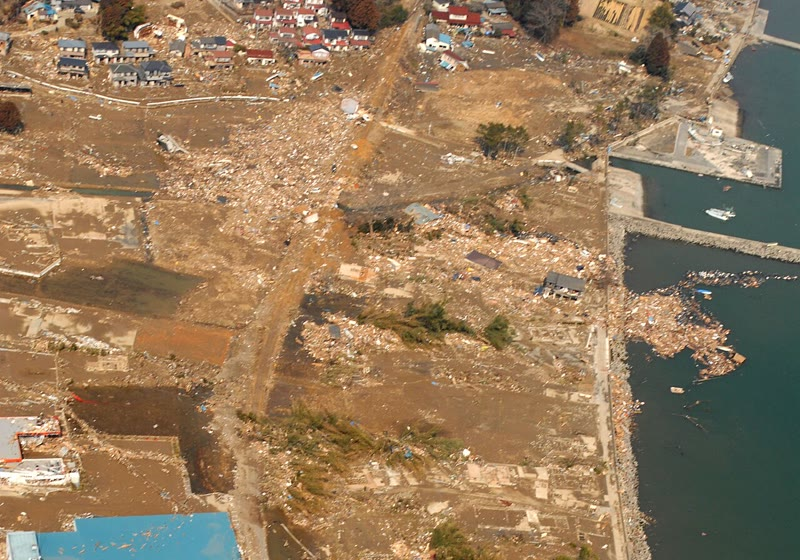
\includegraphics[width=0.78\linewidth]{images/book2/g11-usn-tsunami-kesennuma.jpg}

{\small The fishing port of Kesennuma, on the north-east coast of Japan, two
days after the tsunami of 11~March 2011. Photograph Dylan McCord, U.S. Navy
(public domain).}
\end{omfigure}
% ledger: photo:g11-tsunami

\section{Exercises}

\begin{exercise}[$\star$]\label{exo:g11:subduction-zones:1}
Define \omterm{def:g11:subduction-zones:subduction}{subduction} and a \omterm{def:g11:subduction-zones:subduction}{subduction zone}. Which kind of \omterm{def:g11:lithosphere-asthenosphere:lithosphere}{lithosphere} sinks at a
\omterm{def:g11:subduction-zones:subduction}{subduction zone}, and why that kind?
\end{exercise}

\begin{exercise}[$\star$]\label{exo:g11:subduction-zones:2}
Using the world map of earthquakes by depth: (1) name three regions with
earthquakes deeper than \qty{300}{km}; (2) on which side of a trench do the
deep earthquakes lie? (3) Along the Mid-Atlantic Ridge, how deep are the
earthquakes?
\end{exercise}

\begin{exercise}[$\star$]\label{exo:g11:subduction-zones:3}
The catalogue holds \num{7031} earthquakes of magnitude 6 or more, of which
\qty{21}{\percent} are deeper than \qty{70}{km} and \qty{6.9}{\percent} deeper
than \qty{300}{km}. How many earthquakes is that in each case?
\end{exercise}

\begin{exercise}[$\star$]\label{exo:g11:subduction-zones:4}
Define \omterm{def:g11:subduction-zones:eclogite}{blueschist} and \omterm{def:g11:subduction-zones:eclogite}{eclogite}. What do both have in common with the basalt
of the \omterm{def:g11:ocean-ridges:oceanic-lithosphere}{oceanic crust}? What differs?
\end{exercise}

\begin{exercise}[$\star$]\label{exo:g11:subduction-zones:5}
List the parts of a \omterm{def:g11:subduction-zones:subduction}{subduction zone} in order, from the ocean floor that
moves toward the trench to the back-arc, saying in one line what happens in
each.
\end{exercise}

\begin{exercise}[$\star\star$]\label{exo:g11:subduction-zones:6}
On the Andes section, the line that follows the earthquakes passes
\qty{135}{km} down at \qty{300}{km} from the trench and \qty{508}{km} down at
\qty{800}{km}. Compute the dip of the \omterm{def:g11:subduction-zones:slab}{slab}.
\end{exercise}

\begin{exercise}[$\star\star$]\label{exo:g11:subduction-zones:7}
A straight \omterm{def:g11:subduction-zones:slab}{slab} starts at a trench and dips at \ang{45}. (1) How deep is it
\qty{300}{km} from the trench? (2) At what distance from the trench does it
reach \qty{670}{km}? (3) What length of \omterm{def:g11:subduction-zones:slab}{slab} lies between the trench and
\qty{670}{km}?
\end{exercise}

\begin{exercise}[$\star\star$]\label{exo:g11:subduction-zones:8}
The mean speeds of the plates are, in millimetres a year: Cocos 74.6, Nazca
70.0, Pacific 65.5, Australia 63.1, Philippine Sea 52.6 (with \omterm{def:g11:subduction-zones:slab}{slabs}); Arabia
47.6, Somalia 31.0, Nubia 29.2, Eurasia 22.8, North America 19.8, Antarctica
15.2, Caribbean 14.9, South America 10.6 (without). (1) Compute the mean of
each group and their ratio. (2) What does this suggest about the force that
drives plates?
\end{exercise}

\begin{exercise}[$\star\star$]\label{exo:g11:subduction-zones:9}
In 2011 the fault off Japan slipped by as much as 50 to \qty{60}{m}. The
Pacific plate approaches at \qty{83}{mm} a year. (1) How many years of plate
motion does a slip of \qty{50}{m}, then \qty{60}{m}, make up? (2) Compare with
the time since 869, a possible earlier earthquake of the same size.
\end{exercise}

\begin{exercise}[$\star\star$]\label{exo:g11:subduction-zones:10}
The ocean floor that reaches the Japan Trench is about 133 million years old,
that reaching Tonga about 99 and that reaching the Andes about 49. (1) Using
the laws of \cref{ch:g11:ocean-ridges} ($2500 + 350\sqrt{t}$ for
$t \le 70$, $6400 - 3200\,e^{-t/62.8}$ beyond), find the depth of each. (2)
Which is the coldest and densest \omterm{def:g11:lithosphere-asthenosphere:lithosphere}{lithosphere}?
\end{exercise}

\begin{exercise}[$\star\star$]\label{exo:g11:subduction-zones:11}
The basalt of the \omterm{def:g11:ocean-ridges:oceanic-lithosphere}{oceanic crust} has a density of about \qty{2900}{kg/m^3},
the mantle around the \omterm{def:g11:subduction-zones:slab}{slab} \qty{3380}{kg/m^3}, and \omterm{def:g11:subduction-zones:eclogite}{eclogite} is
\qty{6}{\percent} denser than the mantle. (1) Find the density of \omterm{def:g11:subduction-zones:eclogite}{eclogite}.
(2) By what percentage does the density of the crust rise when it turns into
\omterm{def:g11:subduction-zones:eclogite}{eclogite}? (3) Before and after, is the crust lighter or denser than the
mantle, and by how much?
\end{exercise}

\begin{exercise}[$\star\star\star$]\label{exo:g11:subduction-zones:12}
Heat spreads by conduction over a distance of about $\sqrt{\kappa t}$ in a
time $t$, with $\kappa = \qty{1e-6}{m^2/s}$ for rock. (1) Compute this distance
for 6 million years ($1~\text{year} \approx \qty{3.16e7}{s}$). (2) Compare it
with the thickness of a \omterm{def:g11:subduction-zones:slab}{slab}, about \qty{100}{km}. (3) Explain why
earthquakes can happen inside a \omterm{def:g11:subduction-zones:slab}{slab} at \qty{600}{km} while the mantle around
it flows.
\end{exercise}
% ledger: england:kelvin (kappa 1e-6 m2/s)

\begin{exercise}[$\star\star\star$]\label{exo:g11:subduction-zones:13}
Beneath the Andes at \ang{21}~South, the line of the section reaches
\qty{670}{km} at \qty{1017}{km} from the trench, and the plates converge at
\qty{64}{mm} a year. (1) Estimate the length of \omterm{def:g11:subduction-zones:slab}{slab} from the trench to
\qty{670}{km}. (2) How long does a piece of ocean floor take to reach
\qty{670}{km}? (3) Compare with Tonga, where the same journey takes about 6
million years.
\end{exercise}

\begin{exercise}[$\star\star\star$]\label{exo:g11:subduction-zones:14}
Take a \omterm{def:g11:subduction-zones:slab}{slab} \qty{100}{km} thick, denser than the mantle around it by
\qty{36}{kg/m^3} on average, and \qty{1000}{km} long, beneath a trench.
(1) Compute the mass excess of the \omterm{def:g11:subduction-zones:slab}{slab} for each metre of trench. (2) Compute
its weight, with $g = \qty{9.8}{m/s^2}$. (3) Why can this force pull the whole
plate?
\end{exercise}

\begin{exercise}[$\star\star\star$]\label{exo:g11:subduction-zones:15}
Along the Tonga Trench the PB2002 model gives a convergence of
\qty{104}{mm} a year at \ang{23.6}~South and \qty{237}{mm} a year at
\ang{16.5}~South. (1) How far apart are the two points, along a meridian
($\ang{1} \approx \qty{111}{km}$)? (2) By how much does the rate grow per
hundred kilometres? (3) The Pacific plate moves at about the same speed at
both points. What must the other side of the trench, the Tonga arc, be doing?
\end{exercise}

\section{Problem: The Tonga Slab}

\begin{problem}[{Weekend problem --- from the trench to \qty{670}{km}}]
\label{pb:g11:subduction-zones:1}
% values: tonga fit -23.568 + 0.91068 x; tonga_rate 168.0 mm/yr; tonga_age 98.8;
% x670 761.6; path 1014; time 6.04 Myr; tonga_maxdepth 670.8 (slab_sections.py);
% MKEA 69 mm/yr (plate_velocities.py); kappa england:kelvin; eclogite hacker03:eclogite
Beneath the Tonga Trench the Pacific plate sinks westward. Use the Tonga
section of this chapter, whose line is $z = -24 + 0.91\,x$ (both in
kilometres, $x$ measured from the trench toward the arc).

\medskip
\noindent\textbf{Part I --- The earthquake section.}
\begin{enumerate}
  \item How deep is the deepest earthquake of the section?
  \item Why are there no deep earthquakes on the ocean side of the trench?
  \item Compute the depth of the line at $x = 300$ and $x = 700$, then the
        dip of the \omterm{def:g11:subduction-zones:slab}{slab}.
  \item At what horizontal distance from the trench is the \omterm{def:g11:subduction-zones:slab}{slab}
        \qty{100}{km} deep? And \qty{400}{km} deep?
  \item The line passes \qty{24}{km} above the trench at $x = 0$. What does
        this tell you about the shape of the \omterm{def:g11:subduction-zones:slab}{slab} near the trench?
\end{enumerate}

\medskip
\noindent\textbf{Part II --- The convergence.}
\begin{enumerate}[resume]
  \item The plates converge across the trench at about \qty{168}{mm} a year.
        Convert to centimetres a year and kilometres per million years.
  \item The Pacific plate moves over Hawaii at about \qty{69}{mm} a year.
        How many times faster is the convergence at Tonga?
  \item Using the sum of relative velocities, explain how the convergence can
        exceed the speed of the Pacific plate.
  \item The floor that reaches the trench is about 99 million years old. How
        deep does it lie (exponential law of \cref{ch:g11:ocean-ridges})?
  \item Why can such a \omterm{def:g11:lithosphere-asthenosphere:lithosphere}{lithosphere} sink on its own?
\end{enumerate}

\medskip
\noindent\textbf{Part III --- Down to \qty{670}{km}.}
\begin{enumerate}[resume]
  \item At what horizontal distance from the trench does the line reach
        \qty{670}{km}?
  \item Estimate the length of the \omterm{def:g11:subduction-zones:slab}{slab} from the trench to that point,
        treating it as straight.
  \item How long does a piece of ocean floor take to travel this length at
        \qty{168}{mm} a year?
  \item How long would it take at the \qty{69}{mm} a year of the Pacific
        plate over Hawaii?
  \item On the way, the crust of the \omterm{def:g11:subduction-zones:slab}{slab} turns into \omterm{def:g11:subduction-zones:eclogite}{eclogite},
        \qty{6}{\percent} denser than the mantle at \qty{3380}{kg/m^3}. What
        is its density, and what does this change for the \omterm{def:g11:subduction-zones:slab}{slab}?
\end{enumerate}

\medskip
\noindent\textbf{Part IV --- A cold slab in a hot mantle.}
\begin{enumerate}[resume]
  \item Over the time of question~13, heat spreads by conduction over about
        $\sqrt{\kappa t}$, with $\kappa = \qty{1e-6}{m^2/s}$. Compute this
        distance.
  \item Compare it with the thickness of the \omterm{def:g11:subduction-zones:slab}{slab}, about \qty{100}{km}. Is
        the \omterm{def:g11:subduction-zones:slab}{slab} still cold inside when it reaches \qty{670}{km}?
  \item Why does this explain the earthquakes at \qty{600}{km} and more
        beneath Tonga?
  \item What change in the mantle did seismic waves reveal near
        \qty{670}{km} (\cref{ch:g11:seismic-structure})?
  \item Conclude: how long does Pacific ocean floor take to go from the Tonga
        Trench down to \qty{670}{km}?
\end{enumerate}
\end{problem}
